\documentclass[12pt]{extarticle}
\usepackage{graphicx} % Required for inserting images
\usepackage{lipsum}
\usepackage{soul}
\usepackage{setspace}
\usepackage{multirow}
\singlespacing

\title{LLM Tool-Use for Travel Booking}
\author{Yuriy Sosnin}
\date{July 2025}

\begin{document}

\maketitle

\section{Introduction}

Many modern open-source LLMs can already handle simple tool-use tasks out of the box, especially when tools are defined using OpenAI-style function schemas \cite{openai}. In particular, larger instruction-tuned models like Qwen2.5-7B-Instruct \cite{qwen25} show near-perfect accuracy on single-turn cases. That said, performance drops quickly for smaller models, and it's unclear how much of that is due to scale vs. alignment training.

In this report, we explore this gap by evaluating two related model families - Qwen2 \cite{qwen2} and Qwen2.5 \cite{qwen25} - at different sizes (0.5B to 7B) on a narrow function-calling task. We limit scope to single-turn queries with all arguments specified, and compare zero-shot performance across models. To make things more interesting, we also fine-tune Qwen2-0.5B-Instruct on a tool-use dataset (APIGen \cite{apigen}), to see if we can recover accuracy with minimal training.

We evaluate on a subset of Berkeley Function-Calling Leaderboard \cite{bfcl} (a standard tool-use benchmark) and a small synthetic dataset for booking queries. Accuracy is measured as exact match with ground truth JSON calls. While not a full agent setup, this gives us a clean way to isolate tool-use behavior without reasoning, dialogue, or orchestration.

\section{Related Works}

Early work on tool use with LLMs mostly focused on showing that it’s possible. Toolformer \cite{toolformer} used self-supervised data collection to train a model to call APIs mid-generation. ReAct \cite{react} and WebGPT \cite{webgpt} demonstrated that reasoning and decision-making with tools was viable, especially with access to external state (like search results or environments). But these approaches were more agent-style and didn’t isolate tool-calling as a standalone behavior.

Later work focused more directly on structured tool use and introduced proper benchmarks. Gorilla \cite{gorilla} and ToolLLM \cite{toolllm} both evaluated open models on JSON-style function calling, and Gorilla introduced what is now the Berkeley Function-Calling Leaderboard (BFCL) \cite{bfcl}, which has become one of the standard benchmarks for the task. More datasets later appeared, like Nexus \cite{nexus} or APIGen \cite{apigen}.

Closed models like GPT-4 \cite{openai}, Claude \cite{claude}, and Gemini \cite{gemini} arguably led the way in terms of real-world function calling, especially in production tools and agents. OpenAI's method of using a standard JSON schema is increasingly becoming standard, with most models turning to follow it instead of inventing something new.

In the newest generation of open models, tool use has become a part of instruction tuning. Qwen2.5 \cite{qwen25}, LLaMA-3 \cite{llama3}, and others explicitly advertise tool-use capabilities, often include it in their system prompts, and report benchmark performance. But details vary - some models support multi-call or tool choice, others don’t — and there’s still a lot of variation in how robust the behavior is, especially at smaller scales.

\section{Task Setup \& Evaluation Metrics}

In this project, we strictly focus on single-turn, zero-shot, OpenAI-style \cite{openai} function calling, without CoT \cite{cot}, ReAct \cite{react}, or any other form of orchestration. We also do not consider underspecified user queries, i.e. where some required field is missing in the context and the LLM call should result in \textit{rejection} (see Discussion). Therefore, we define the following interaction protocol: the system prompt specifies tools available to the model, in JSON Schema format; the user asks something that necessitates the use of at least one of the tools; the model is expected to produce a structured JSON object with function names and parameters.

Although our target application is flight and hotel booking, we believe it is valuable to evaluate on a broad and general tool-use benchmark. We choose Berkeley Function Calling Leaderboard (BFCL) \cite{bfcl}. It consists of multiple different subsets, corresponding to different flavors and difficulty levels of the task. We only use the "simple" and "multiple" subsets, corresponding to one function + one call and multiple functions + one call setups, respectively.

On top of that, we also follow BFCL format to design our own small benchmark focused on the booking domain and our concrete functions. By design, it always has only 2 available functions, and one of 2 intents: hotel or flight. To collect the dataset, we use a common technique of synthetic data collection by reversing the task. Basically, we prompt GPT-4.1-mini with a seed example and the function definition, and ask it to generate both a plausible query and correct ground truth JSON call. There are 20 examples in total, half for hotel booking and the other for flights.

The primary metric used to evaluate this task is tool-calling accuracy: for each example, we compare the model's predicted JSON call(s) to the ground truth, available in advance. Following BFCL, we use AST-based validation - that is, we compare function name, argument structure, and values semantically, rather than relying on exact string match.

\section{Experimental Setup}

To comply with the constraints of the assignment, we limit our study to sub-7b open-source language models. Within this range, we select two related model families: Qwen2 \cite{qwen2} and Qwen2.5 \cite{qwen25}, each released in 0.5b, 1.5b, and 7b variants.

These families provide a useful basis for systematic comparison. First, they allow us to investigate the scaling behavior of tool-use performance as a function of model size. Second, they differ in their alignment strategies: Qwen2.5 models have been explicitly instruction-tuned on tool-use, while Qwen2 models have not (or at least no such training is disclosed). This divergence allows us to isolate the impact of tool-specific alignment, in particular at smaller scales where zero-shot performance is less robust.

In the first stage of our study, we evaluate these models as is, with the default Qwen2.5 system prompt that includes tool definitions in OpenAI-style JSON Schema format. Since Qwen2 does not have a recommended tool-use prompt format, we use the same prompt for it too, for consistency.

We notice that Qwen2-0.5B-Instruct significantly underperforms, nearing 0 accuracy, and decide to fine-tune it, to assess how effective SFT fine-tuning would be for tool use on such a small scale. We use the APIGen Function-Calling Dataset \cite{apigen} - we choose this dataset over OpenFunctions \cite{gorilla} or Nexus \cite{nexus} due to its compatibility with OpenAI-style Schema out of the box. APIGen consists of 60k examples of various Python functions, with multiple available tools and multiple possible calls in each example.

We train a simple LoRA adapter \cite{lora} for one epoch, with the effective batch size of 32 and learning rate of 2e-4. One training run on 1 $\times$ A100 40GB in bf16 precision takes about 40 minutes.

\section{Results}

\begin{table}[h]
\centering
\caption{Model Performance Comparison: Qwen2 vs Qwen2.5 Across Model Sizes}
\begin{tabular}{|l|l|c|c|c|c|c|c|c|}
\hline
\multirow{2}{*}{\textbf{Dataset}} & \multirow{2}{*}{\textbf{Subset}} & \multicolumn{3}{c|}{\textbf{Qwen2}} & \multicolumn{3}{c|}{\textbf{Qwen2.5}} & \textbf{Qwen2-SFT} \\
\cline{3-8}
 &  & \textbf{0.5B} & \textbf{1.5B} & \textbf{7B} & \textbf{0.5B} & \textbf{1.5B} & \textbf{7B} & \textbf{0.5B} \\
\hline
\multirow{2}{*}{bfcl} & simple & 0.045 & 0.6225 & 0.935 & 0.78 & 0.84 & 0.9625 & 0.7475 \\
\cline{2-9}
 & multiple & 0.15 & 0.825 & 0.955 & 0.7 & 0.85 & 0.965 & 0.705 \\
\hline
booking & multiple & 0.1 & 0.85 & 0.85 & 0.35 & 0.8 & 0.75 & 0.5 \\
\hline
\end{tabular}
\label{tab:model_performance}
\end{table}

\begin{figure}[h]
    \centering
    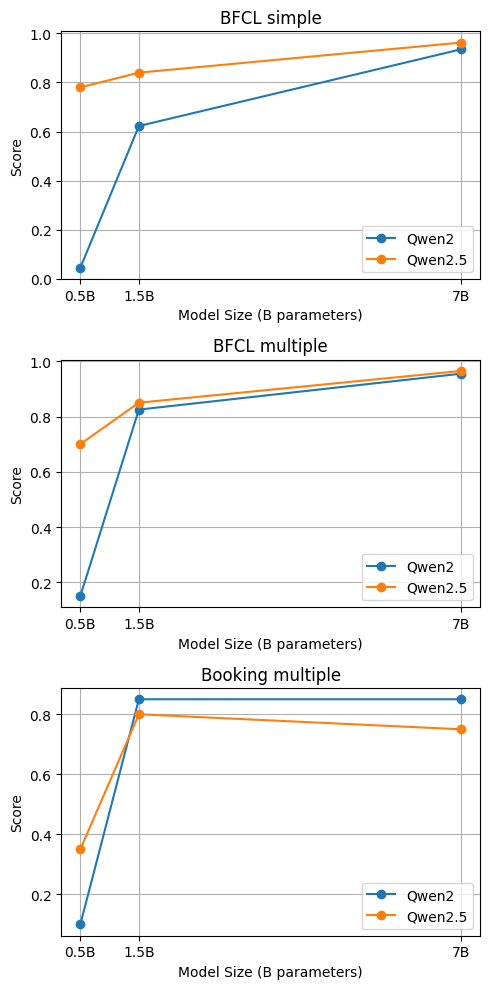
\includegraphics[height=0.95\textheight]{output.png}
    \caption{Model Performance vs Size: Qwen2 vs Qwen2.5 Comparison}
    \label{fig:model_performance}
\end{figure}

With the model families and datasets in place, we proceed to evaluate performance across two experimental stages: (1) zero-shot inference using the base instruction-tuned models, and (2) supervised fine-tuning of a smaller model (Qwen2-0.5B-Instruct) to assess learnability under low-scale alignment. All evaluations use the task and metrics setup described in Section 3. Our experimental results can be examined in Table 1.

Looking at zero-shot performance, one can see that 7B models already perform nearly perfectly - interestingly, both models trained on tool use and not. Additionally, performance drops with model size, but only slightly on Qwen2.5 and significantly on Qwen2. At the smallest model level, 0.5B, performance drops considerably, nearly to zero. However, fine-tuning this model on actual tool-use dataset improves the score dramatically, allowing it to be on par even with Qwen2.5.

While both benchmarks show similar dynamics, our booking benchmark has lower scores and higher variance mostly due to date formatting, which turns out to be difficult for the models to do right.

\section{Limitations \& Discussion}

There are several important setups we explicitly leave out in this report. First, we do not test parallel tool use, where multiple tools are invoked in a single step. While BFCL includes this subset, and we could expand our benchmark with this form too, we focus only on one-call setups for clarity.

More critically, we do not consider multi-turn dialogue, i.e. feeding the tool result back into the model and expecting either further tool use or natural language output. We also do not test reasoning before calling (e.g., CoT or ReAct-style prompting), nor any form of state tracking.

We also leave multilingual evaluation out. Many recent models claim some level of non-English coverage (especially Qwen), and testing, for example, Russian inputs could have been an interesting axis.

Finally, a major open question - in our work and in the literature - is evaluating \textit{rejections}. That is: can a model recognize when it lacks context to call a tool, and choose to do nothing (or ask a follow-up), especially in ambiguous cases? Anecdotally, the Qwen models we tested tend to hallucinate missing parameters instead. One way to deal with the problem would be to define a synthetic "reject" tool explicitly - something we did not explore, but which would make rejection measurable under the same metric.

\section{Conclusion}

We explored tool-use capabilities of sub-7B instruction-tuned models in a simplified single-turn setting. By comparing Qwen2 and Qwen2.5 families across sizes and running a small fine-tuning experiment on Qwen2-0.5B-Instruct, we showed how scale and alignment both affect performance.

Out-of-the-box results on BFCL and a custom booking benchmark confirmed that tool-specific alignment matters most at smaller scales, but becomes less important at 7B. A single LoRA fine-tune was enough to recover most of the gap for a small unaligned model.

\bibliographystyle{plain}
\bibliography{main}

\end{document}
